% ---------------------------------------------
% SNUDM Center Technical Report Template (2015)
% http://dm.snu.ac.kr
% ---------------------------------------------

% Set parameters
\documentclass[11pt]{article}           % set fontsize

\renewcommand{\baselinestretch}{1.3}    % set line height
\renewcommand{\today}{April 14, 2015}   % TODO: set date
\usepackage{geometry}                   % set margin
    \geometry{a4paper, left=20mm, right=20mm, top=25mm, bottom=25mm}
\usepackage{kotex}                      % in case you use Korean
    \renewcommand{\figurename}{그림}    % delete for English documents
    \renewcommand{\tablename}{표}       % delete for English documents
    \renewcommand{\refname}{참고문헌}   % delete for English documents
\usepackage{graphicx}                   % for png images
\usepackage{hyperref}                   % for urls
\usepackage{fancyhdr}                   % for header (should come after hyperref)
    \fancypagestyle{plain} {
        \fancyhf{}
        \fancyhead[L]{
            \href{http://dm.snu.ac.kr}{SNU Data Mining Center}
        }
        \fancyhead[R]{SNUDM-TR-2015-01} % TODO
    }

% Begin document
\begin{document}
\title{\LaTeX Template for SNUDM Technical Reports}
\author{
  조성준\\
  \texttt{zoon@snu.ac.kr}
  \and
  홍길동\\
  \texttt{hong@dm.snu.ac.kr}
}
\maketitle

\begin{abstract}
This article demonstrates a basic set of LaTeX formatting commands.
Compare the typeset output side-by-side with the input document.
\end{abstract}

\section{서론}
텍스트는 길고 자유롭게 입력할 수 있다.
    들여쓰기나 띄어쓰기를 어떻게 해도
  \LaTeX이 알아서 깔끔하게 출력해줄 것이니, 원고를 편리하게 포맷팅할 수 있다.
보통은 한 문장 혹은 한 구절을 한 줄에 입력한다.

다만 엔터키를 두 번 입력해서 빈칸을 입력하면 단락이 나눠진다는 것은 알아두자.
텍스트를 강조하는 방법은 아주 다양하지만 \textit{주로 이탤릭체나} \textbf{볼드체로} 표기하는 것이 일반적이다.

`작은 따옴표'나 ``큰 따옴표''를 쓸때는 조심해야 한다.
왼쪽과 오른쪽에 사용하는 문자가 다르기 때문이다.
누군가를 인용하거나 들여쓰기를 할 때는 \verb+quotation+ 환경을 쓰면 된다:

\begin{quotation}
Data mining (the analysis step of the "Knowledge Discovery in Databases" process, or KDD), an interdisciplinary subfield of computer science, is the computational process of discovering patterns in large data sets involving methods at the intersection of artificial intelligence, machine learning, statistics, and database systems.~\cite{mucha2010community}
\end{quotation}

\subsection{이것은 절입니다}

지금까지 제목과 장/절 입력, 단락 나누기, 텍스트 강조하기, 인용 등을 살펴보았다.
다음으로 목록과 표, 그림 입력에 관해 알아보자.
\footnotemark[1]
\footnotetext[1]{이 문서의 코드는 http://github.com/snudm/dmtr에서 찾으실 수 있습니다.}

\begin{enumerate}
    \item 이렇게
    \item 숫자 목록을 생성하거나
\end{enumerate}

\begin{itemize}
   \item 이렇게
   \item 점 목록을 생성할 수 있다.
\end{itemize}

표는 아래의 표 \ref{tab:backpacking}과 같이 입력한다.

\begin{table}
\centering
    \begin{tabular}{|l|c|p{3.5in}|}
    \hline
    \multicolumn{3}{|c|}{Places to Go Backpacking}\\ \hline
    Name    & Driving Time  & Notes\\
            & (hours)       & \\ \hline
    Big     & 1.5           & Very nice overnight to Berry Creek Falls from
    either Headquarters or oean side.\\ \hline
    Sunol   & 1             & Technicolor green in the spring. Watch out for the cows.\\ \hline
    Henry   & 1.5           & Large wilderness nearby suitable for multi-day treks.\\ \hline
    \end{tabular}
    \caption{Places to go backpacking}
    \label{tab:backpacking}
\end{table}

그림은 아래의 그림 \ref{fig:sankey}과 같이 이미지 파일로 입력하거나 
\verb+tikz+를 이용해서 \LaTeX으로 직접 조판할 수 있다.

\begin{figure}[t]
    \centering
    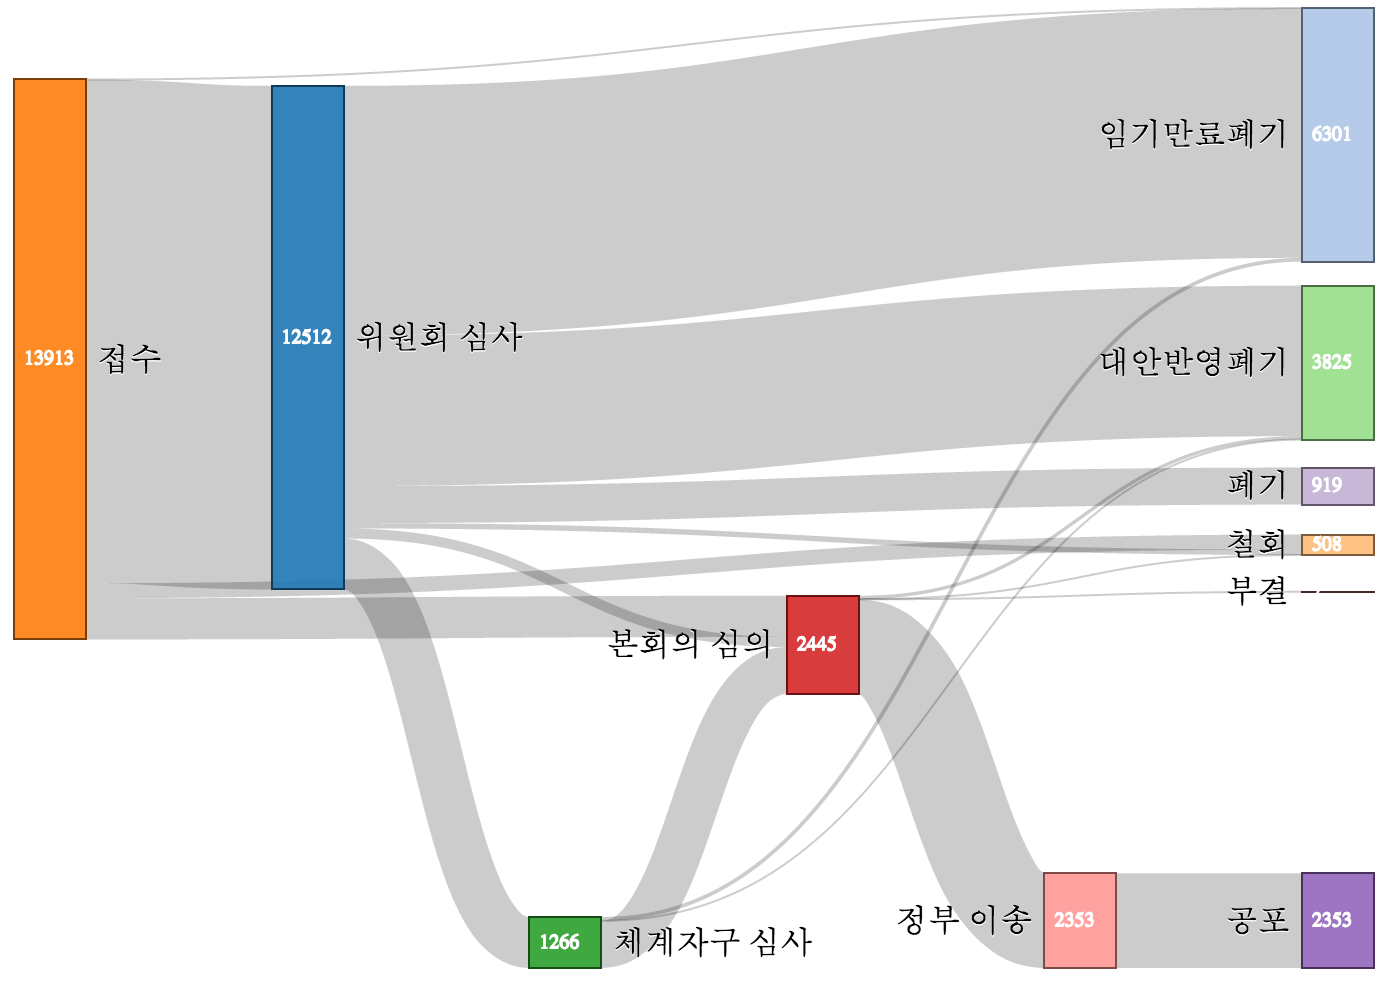
\includegraphics[width=0.7\textwidth]{sankey.png}
    \caption{하하하}
    \label{fig:sankey}
\end{figure}

\section{수식 입력}
$x^y$ 또는 $x_n = \sqrt{a + b}$과 같이 간단한 수식은 달러 기호를 이용해서 인라인(inline)으로 바로 입력할 수 있다.
실제로 \$2000 이렇게 달러 기호를 조판하고 싶다면 \verb+\$2000+와 같이 달러 기호를 escaping해주면 된다.

더 복잡한 수식을 입력하는 경우에는 두 가지 방법이 있다.
먼저, 수식에 번호를 달지 않고 수식을 입력하는 법:

\[
    z \left( 1 \ +\  \sqrt{\omega_{i+1} + \zeta -\frac{x+1}{\Theta +1} y + 1} 
    \ \right)
    \ \ \ =\ \ \  1
\]

다음으로 수식에 번호를 달고 입력하는 법:

\begin{equation}
    \left[
    {\bf X} + {\rm a} \ \geq\ 
    \underline{\hat a} \sum_i^N \lim_{x \rightarrow k} \delta C
    \right]
\end{equation}

끝으로, 참고문헌을 불러오고 문서를 닫아주는 것을 잊지 말자.

\bibliographystyle{plain}
\bibliography{ref}

\end{document}
